\section{GM-9. Builder}

\subsection*{Problema}
Un constructor con varios números facilitaría confundir objetivo, velocidad, intervalo y probabilidad.

\subsection*{Contexto}
Cada dificultad construye configuraciones para 30 niveles; se necesitan valores válidos e inmutabilidad posterior.

\subsection*{Solución y aplicación}
\texttt{Nivel.Builder} ofrece métodos encadenables con nombres y valores predeterminados. \texttt{construir()} comprueba nombre, objetivo positivo, velocidad e intervalo positivos y finitos, y probabilidad finita entre 0 y 1. Crea un \texttt{Nivel} con campos privados finales. El cliente real es \texttt{Dificultad.crearNivel()}. No se incorpora un Director porque esta construcción no lo necesita.

\subsection*{Evidencia}
\begin{itemize}
\item \href{https://github.com/maverick1006/Proyecto-Game-LLuvia-/blob/codex/entrega-final/core/src/main/java/puppy/code/Nivel.java#L23}{Nivel.java, línea 23} (\texttt{public static class Builder})
\item \href{https://github.com/maverick1006/Proyecto-Game-LLuvia-/blob/codex/entrega-final/core/src/main/java/puppy/code/Nivel.java#L34}{Nivel.java, línea 34} (\texttt{public Nivel construir()})
\item \href{https://github.com/maverick1006/Proyecto-Game-LLuvia-/blob/codex/entrega-final/core/src/main/java/puppy/code/Nivel.java#L10}{Nivel.java, línea 10} (\texttt{private Nivel(Builder b)})
\item \href{https://github.com/maverick1006/Proyecto-Game-LLuvia-/blob/codex/entrega-final/core/src/main/java/puppy/code/Dificultad.java#L16}{Dificultad.java, línea 16} (\texttt{public Nivel crearNivel(})
\end{itemize}

\subsection*{UML}
\begin{figure}[htbp]
\centering
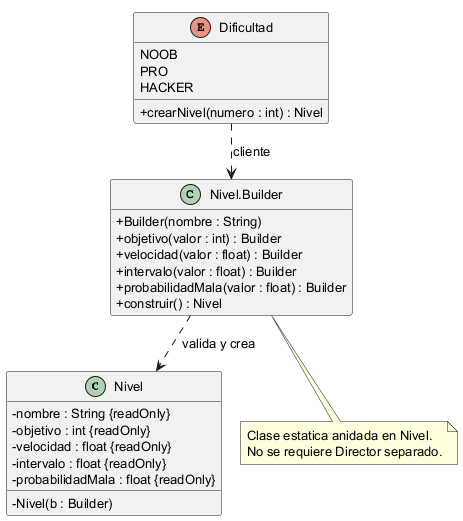
\includegraphics[width=0.95\linewidth,height=0.72\textheight,keepaspectratio]{images/05-builder.png}
\caption{05 builder}
\end{figure}




